\documentclass{article}
\usepackage[utf8]{inputenc}
\usepackage{feynmf}
\usepackage{pgfplots}
\usepackage{graphicx}
%\usepackage{subfigure}
\usepackage{subcaption}
\usepackage{caption}
\usepackage[T1]{fontenc} % Output font encoding for international characters
\usepackage[justification=centering]{caption}
\pgfplotsset{compat=1.15}

\title{SM Feynman Diagrams}
\author{chazinb}
\date{June 2019}


\begin{document}

% Define some commands to keep the formatting separated from the content 
\newcommand{\keyword}[1]{\textbf{#1}}
\newcommand{\tabhead}[1]{\textbf{#1}}
\newcommand{\code}[1]{\texttt{#1}}
\newcommand{\file}[1]{\texttt{\bfseries#1}}
\newcommand{\option}[1]{\texttt{\itshape#1}}
\setlength{\parskip}{3mm}
%\usepackage{color}

%----------------------------------------------------------------------------------------

\maketitle

%\section{Introduction} % Main chapter title

\label{SectionIntro} % For referencing the chapter elsewhere, use \ref{Chapter1} 

In the beginning of the document ... we had an empty screen, but after some work, we get... the LO Feynman diagrams for SM-processes production in proton-proton collisions 

some references: https://wiki.physik.uzh.ch/cms/latex:feynman


\clearpage
\section{Top backgrounds} % Main chapter title

\label{SectionTop} % For referencing the chapter elsewhere, use \ref{Chapter1} 




%%%%%%%%%%%%%%%%%%%%%%%%%%%%%%%%%%%%%%%%%%%%%%%%%%%%%%%%%%%%
\subsection{LO diagrams for ST production} 
%%%%%%%%%%%%%%%%%%%%%%%%%%%%%%%%%%%%%%%%%%%%%%%%%%%%%%%%%%%%

\vspace{7mm}

    \begin{figure}[h]
    \centering
    \begin{fmffile}{ST-tchannel}
    \begin{fmfgraph*}(100,80)
    % # ins/outs
    \fmfstraight
    \fmftop{i2,v2,o2}
    \fmfbottom{i1,v1,o1}
    % ins
    \fmf{fermion}{i2,v2}
    \fmf{fermion}{i1,v1}
    \fmflabel{q}{i2}
    \fmflabel{$b$}{i1}
    % mediators 
    \fmf{photon, label=$W^*$}{v1,v2}
    % outs
    \fmf{fermion}{v2,o2}
    \fmf{fermion}{v1,o1}
    \fmflabel{$q'$}{o2}
    \fmflabel{$t$}{o1}
    \fmfdotn{v}{2}
    \end{fmfgraph*}  
    \end{fmffile}
    \vspace{3mm}
    \caption{}
    \label{fig:ST_tchannel}
    \end{figure}
    \vspace{7mm}
    
    \begin{figure}[h]
    \centering
    \begin{fmffile}{ST-schannel}
    \begin{fmfgraph*}(100,80)
    % # ins/outs
    \fmfleft{i1,i2}
    \fmfright{o1,o2}
    % ins
    \fmf{fermion}{v1,i2}
    \fmf{fermion}{i1,v1}
    \fmflabel{$\overline{q}$}{i2}
    \fmflabel{$q'$}{i1}
    % mediators 
    \fmf{photon, label=$W^+$}{v1,v2}
    % outs
    \fmf{fermion}{v2,o2}
    \fmf{fermion}{o1,v2}
    \fmflabel{$t$}{o2}
    \fmflabel{$\overline{b}$}{o1}
    \end{fmfgraph*}  
    \end{fmffile}
    \vspace{3mm}
    \caption{}
    \label{fig:ST_schannel}
    \end{figure}
    \vspace{7mm}
    
    \begin{figure}[h]
    \centering
    \begin{fmffile}{ST-tWa}
    \begin{fmfgraph*}(100,80)
    % # ins/outs
    \fmfright{o1,o2}
    \fmfleft {i1,i2}
    % ins
    \fmf{gluon}{i2,v2}
    \fmf{fermion}{i1,v1}
    \fmflabel{g}{i2}
    \fmflabel{$b$}{i1}
    % mediators 
    \fmf{fermion, label=$t$}{v1,v2}
    % outs
    \fmf{fermion}{v2,o2}
    \fmf{photon}{v1,o1}
    \fmflabel{$t$}{o2}
    \fmflabel{$W^-$}{o1}
    \end{fmfgraph*}  
    \end{fmffile}
    \caption{}
    \label{fig:ST_tWa}
    \end{figure}
    \vspace{7mm}
    
    \begin{figure}[h]
     \centering
      \begin{fmffile}{ST-tWb}
    \begin{fmfgraph*}(100,80)
    % # ins/outs
    \fmfleft{i1,i2}
    \fmfright{o1,o2}
    % ins
    \fmf{gluon}{i2,v1}
    \fmf{fermion}{i1,v1}
    \fmflabel{g}{i2}
    \fmflabel{$b$}{i1}
    % mediators 
    \fmf{fermion, label=$b$}{v1,v2}
    % outs
    \fmf{fermion}{v2,o2}
    \fmf{photon}{v2,o1}
    \fmflabel{$t$}{o2}
    \fmflabel{$W^-$}{o1}
    \end{fmfgraph*}  
    \end{fmffile}
    \vspace{3mm}
    \caption{}
    \label{fig:ST_tWb}
    \end{figure}
    \vspace{7mm}



%%%%%%%%%%%%%%%%%%%%%%%%%%%%%%%%%%%%%%%%%%%%%%%%%%%%%%%%%%%%
\subsection{LO diagrams for ttbar production} 
%%%%%%%%%%%%%%%%%%%%%%%%%%%%%%%%%%%%%%%%%%%%%%%%%%%%%%%%%%%%

\vspace{7mm}

% qq->ttbar ; gg->ttbar


% ============
%  s-channel  
% ============
\begin{figure}[h]
%\subfigure[s-channel]{
\centering
\begin{fmffile}{ttbar-schannel}
  \begin{fmfgraph*}(100,80)
    % # in/out
    \fmfleft{i1,i2}
    \fmfright{o1,o2}    
    % ins
    \fmf{gluon}{i1,v1}
    \fmf{gluon}{i2,v1}
    \fmflabel{\(g\)}{i1}
    \fmflabel{\(g\)}{i2}
    % mediators    
    \fmf{gluon, label= $g$, label.dist=5mm}{v1,v2}
    % outs
    \fmf{fermion}{v2,o2}
    \fmflabel{$t$}{o2}
    \fmf{fermion}{o1,v2}
    \fmflabel{$\overline{t}$}{o1}
\end{fmfgraph*}
\end{fmffile}
\vspace{3mm}
\caption{}
\label{fig:ttbar_schannel}
\end{figure}
\vspace{7mm}

\begin{figure}[h]
%\vspace{3mm}
%\hspace{4mm}
% ============
%  t-channel  
% ============
%\subfigure[t-channel]{
\centering
\begin{fmffile}{ttbar-tchannel}
  \begin{fmfgraph*}(100,80)
    % # in/out
     \fmfbottom{i1,d1,o1}
    \fmftop{i2,d2,o2}
    %\fmfleft{i1,i2}
    %\fmfright{o1,o2}
    % ins     
    \fmf{gluon}{i1,v1}
    \fmf{gluon}{i2,v2}
    \fmflabel{\(g\)}{i1}
    \fmflabel{\(g\)}{i2}
    % mediators
    \fmf{fermion, label=$t$, tension=0}{v1,v2}
    % outs
    \fmf{fermion}{o1,v1}
    \fmflabel{$\overline{t}$}{o1}
    \fmf{fermion}{v2,o2}
    \fmflabel{$t$}{o2}
   \end{fmfgraph*}
   %\hspace{2em}
\end{fmffile}
\vspace{3mm}
%}
\caption{}
\label{fig:ttbar_tchannel}
\end{figure}
\vspace{7mm}

% ============
%  u-channel  
% ============
\begin{figure}[h]
\centering
\begin{fmffile}{cross}
  \begin{fmfgraph*}(100,80)
    \fmfleft{i1,i2}
    \fmfright{o1,o2}
    % ins
    \fmf{gluon}{i1,v1}
    \fmf{phantom}{v1,o1} % invisible
    \fmf{gluon}{i2,v2}
    \fmf{phantom}{v2,o2} % invisible
    \fmflabel{\(g\)}{i1}
    \fmflabel{\(g\)}{i2}
    % mediators    
    \fmf{fermion, label= $t$}{v2,v1} 
    % outs
    \fmf{fermion, tension=0}{o1,v2}
    \fmflabel{$\overline{t}$}{o1}
    \fmf{fermion, tension=0}{v1,o2}
    \fmflabel{$t$}{o2}
\end{fmfgraph*}
\end{fmffile}
%}arrow_len
\vspace{3mm}
\caption{}
\label{fig:ttbar_uchannel}
\end{figure}
\vspace{7mm}

\begin{figure}[h]
% =================
%  qq-annihilation  
% =================
\centering
\begin{fmffile}{ttbar-annihilation}
  \begin{fmfgraph*}(100,80)
    % # in/out
    \fmfleft{i1,i2}
    \fmfright{o1,o2}    
    % ins
    \fmf{fermion}{i1,v1}
    \fmf{fermion}{v1,i2}
    \fmflabel{\(q\)}{i1}
    \fmflabel{\(\overline{q}\)}{i2}
    % mediators    
    \fmf{gluon, label.dist=5mm, label= $g$}{v1,v2}
    % outs
    \fmf{fermion}{v2,o2}
    \fmflabel{$t$}{o2}
    \fmf{fermion}{o1,v2}
    \fmflabel{$\overline{t}$}{o1}
\end{fmfgraph*}
\end{fmffile}
\vspace{3mm}
%}
\caption{}
\label{fig:ttbar_qqttar}
\end{figure}
\vspace{7mm}


%%%%%%%%%%%%%%%%%%%%%%%%%%%%%%%%%%%%%%%%%%%%%%%%%%%%%%%%%%%%
\subsection{ The ttbar decays} 
%%%%%%%%%%%%%%%%%%%%%%%%%%%%%%%%%%%%%%%%%%%%%%%%%%%%%%%%%%%%
\vspace{7mm}
\begin{figure}[h]
    \centering
\begin{fmffile}{tt2l}
  \begin{fmfgraph*}(180,150)
    \fmfset{arrow_len}{3.5mm}
    \fmfstraight
    \fmfleft{i1,i2,i3,i4,i5}
    \fmfright{o1,o2,o3,o4,o5,o6}
    % bW -> bqq
    \fmf{boson,tension=1.5,label={$W^+$},label.side=right}{v2,v21}  % W boson
    \fmf{fermion}{v2,o6}     % b quark
    \fmf{fermion}{o5,v21,o4}
    % bW -> blnu
    \fmf{boson,tension=1.5,label={$W^-$},label.side=right}{v1,v11}  % W boson
    \fmf{fermion}{o3,v1}     % bbar quark
    \fmf{fermion}{o1,v11,o2}
    \fmf{fermion,tension=1.5}{v1,i3,v2}  % top quark pair
    \fmf{phantom,label={$\overline{t}$},tension=1,label.side=rigth}{i3,v1}
    \fmf{phantom,label={$t$},tension=1,label.side=left}{i3,v2}
    \fmflabel{$ \overline{q}' / \overline{\nu}_{\ell}  $}{o1}
    \fmflabel{$ q / \ell^-$}{o2}
    \fmflabel{$\overline{b}$}{o3}
    \fmflabel{$ q / \nu_\ell   $}{o4}
    \fmflabel{$\overline{q}' / \ell^+$}{o5}
    \fmflabel{$b$}{o6}
  \end{fmfgraph*}
\end{fmffile}
\vspace{3mm}
    \caption{}
    \label{fig:ttbarLep}
\end{figure}
\vspace{7mm}

\subsection{ ttZ and ttW production}
\vspace{7mm}
\begin{figure}[h]
    \centering
    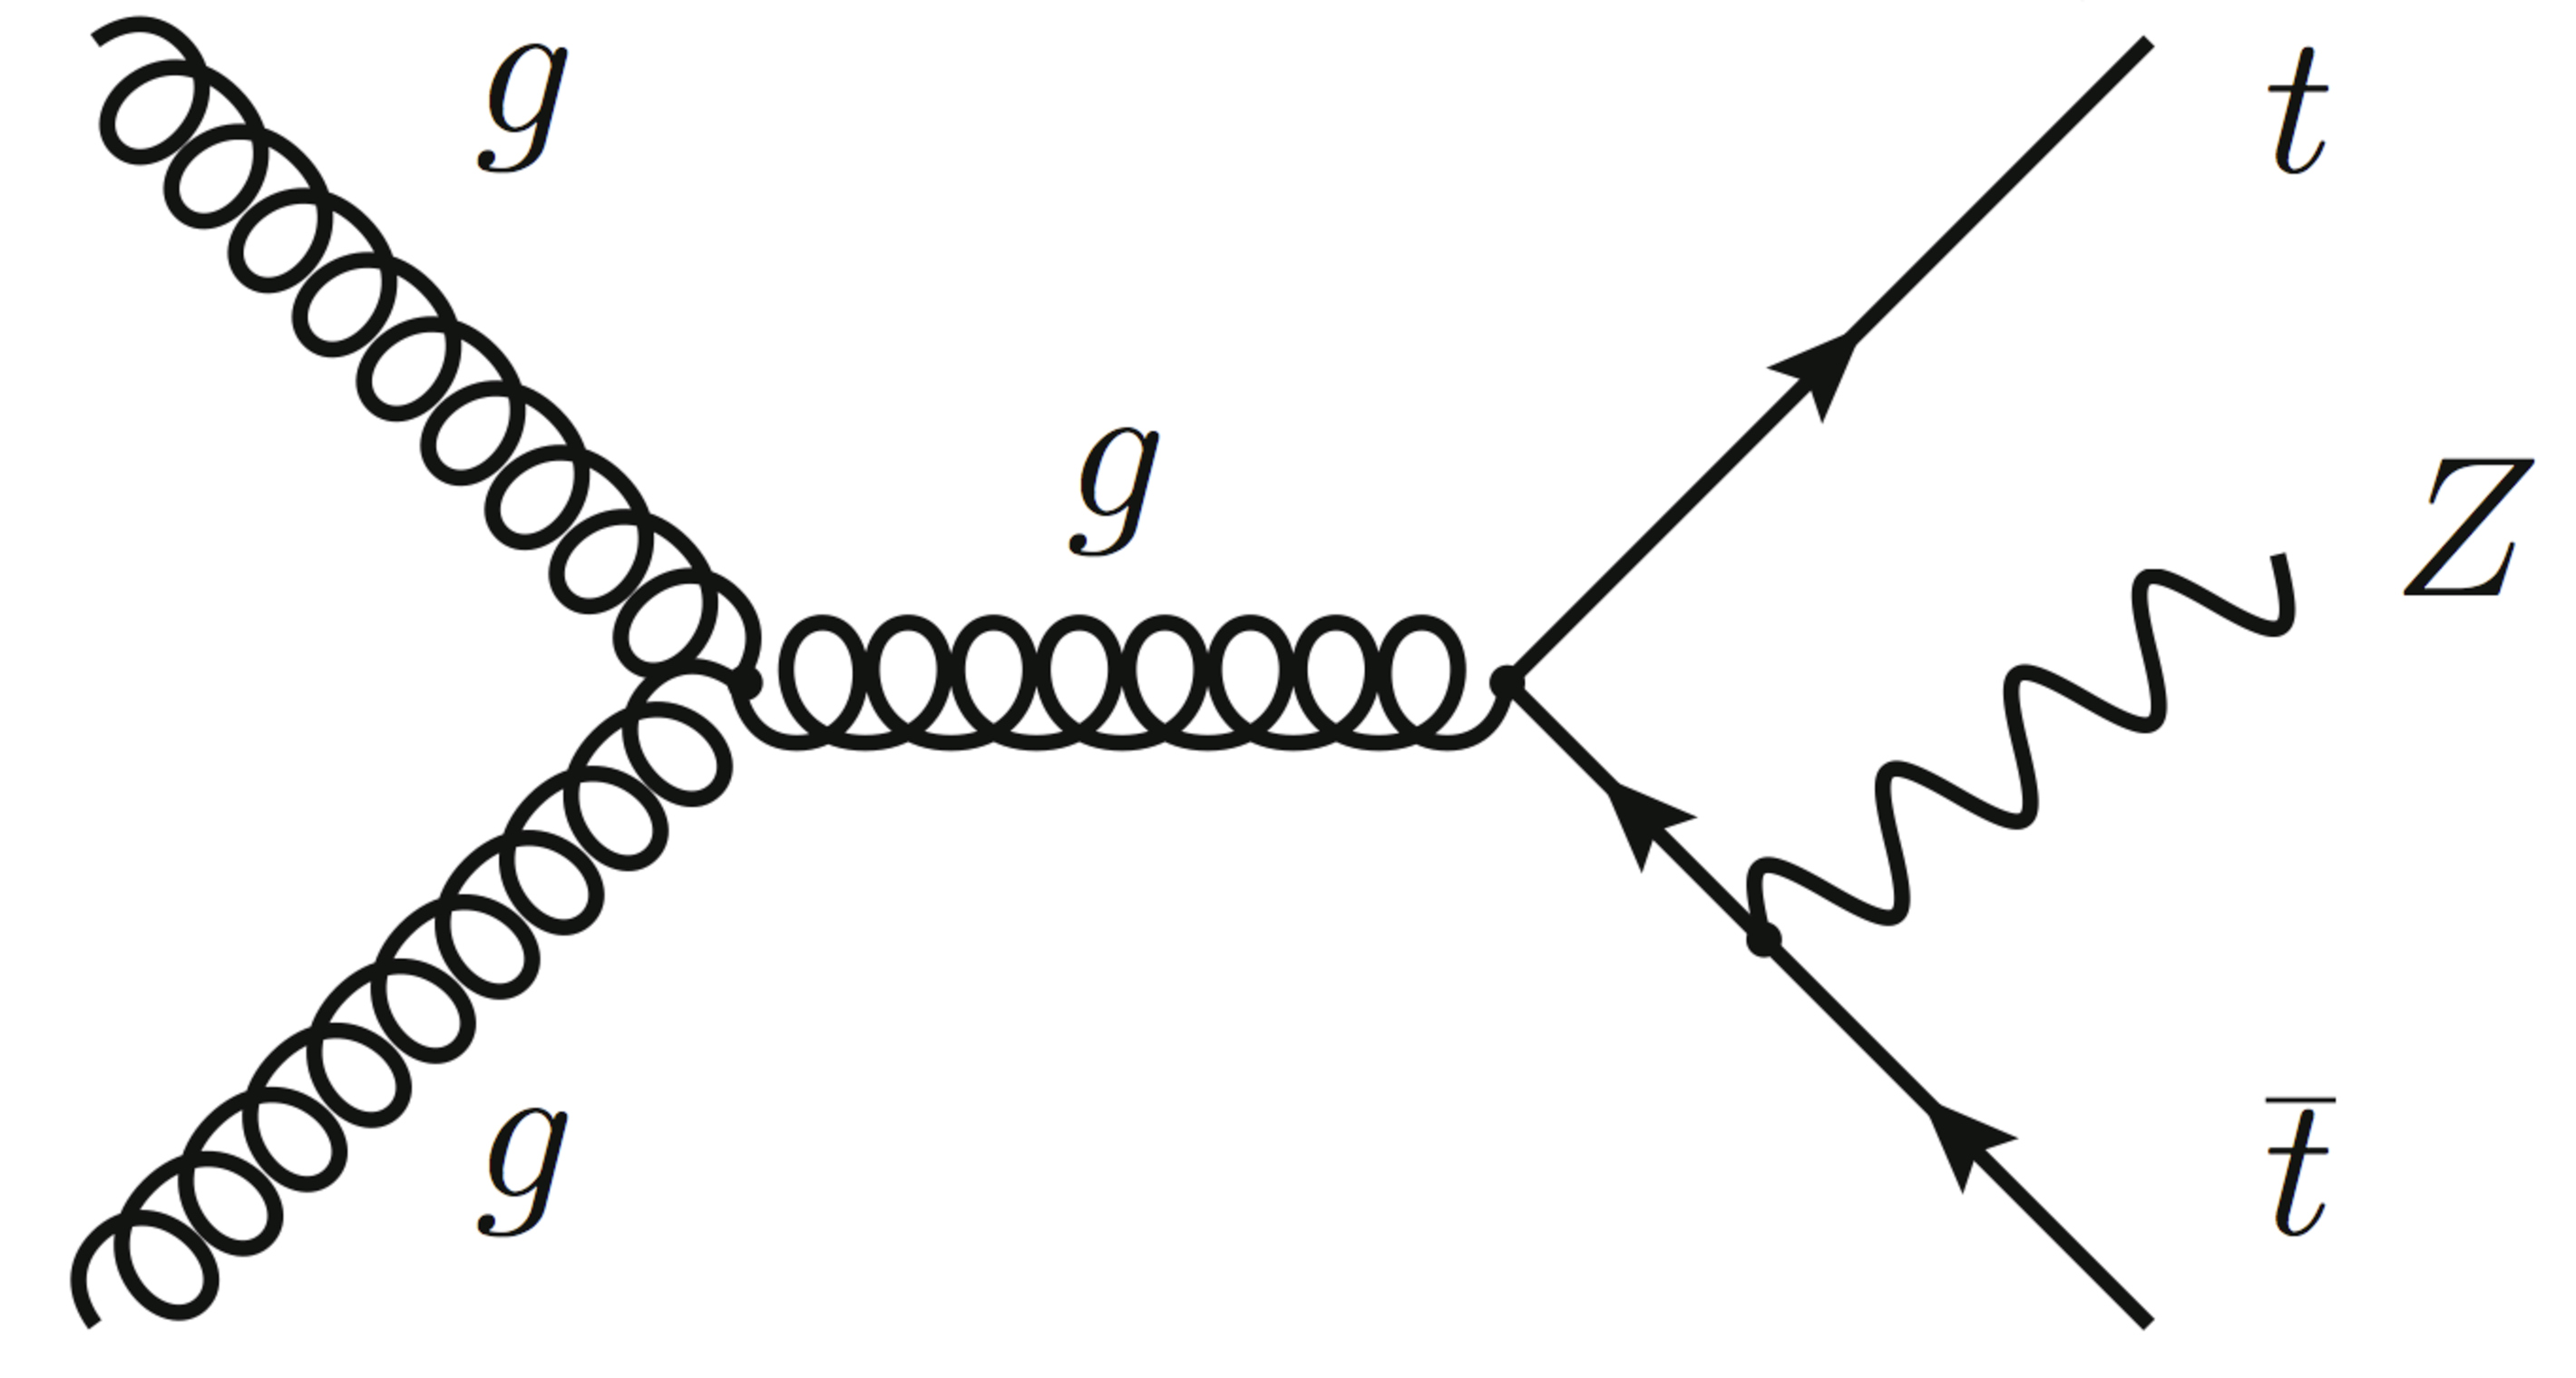
\includegraphics[scale=0.1]{ttZ_feynman.pdf}
    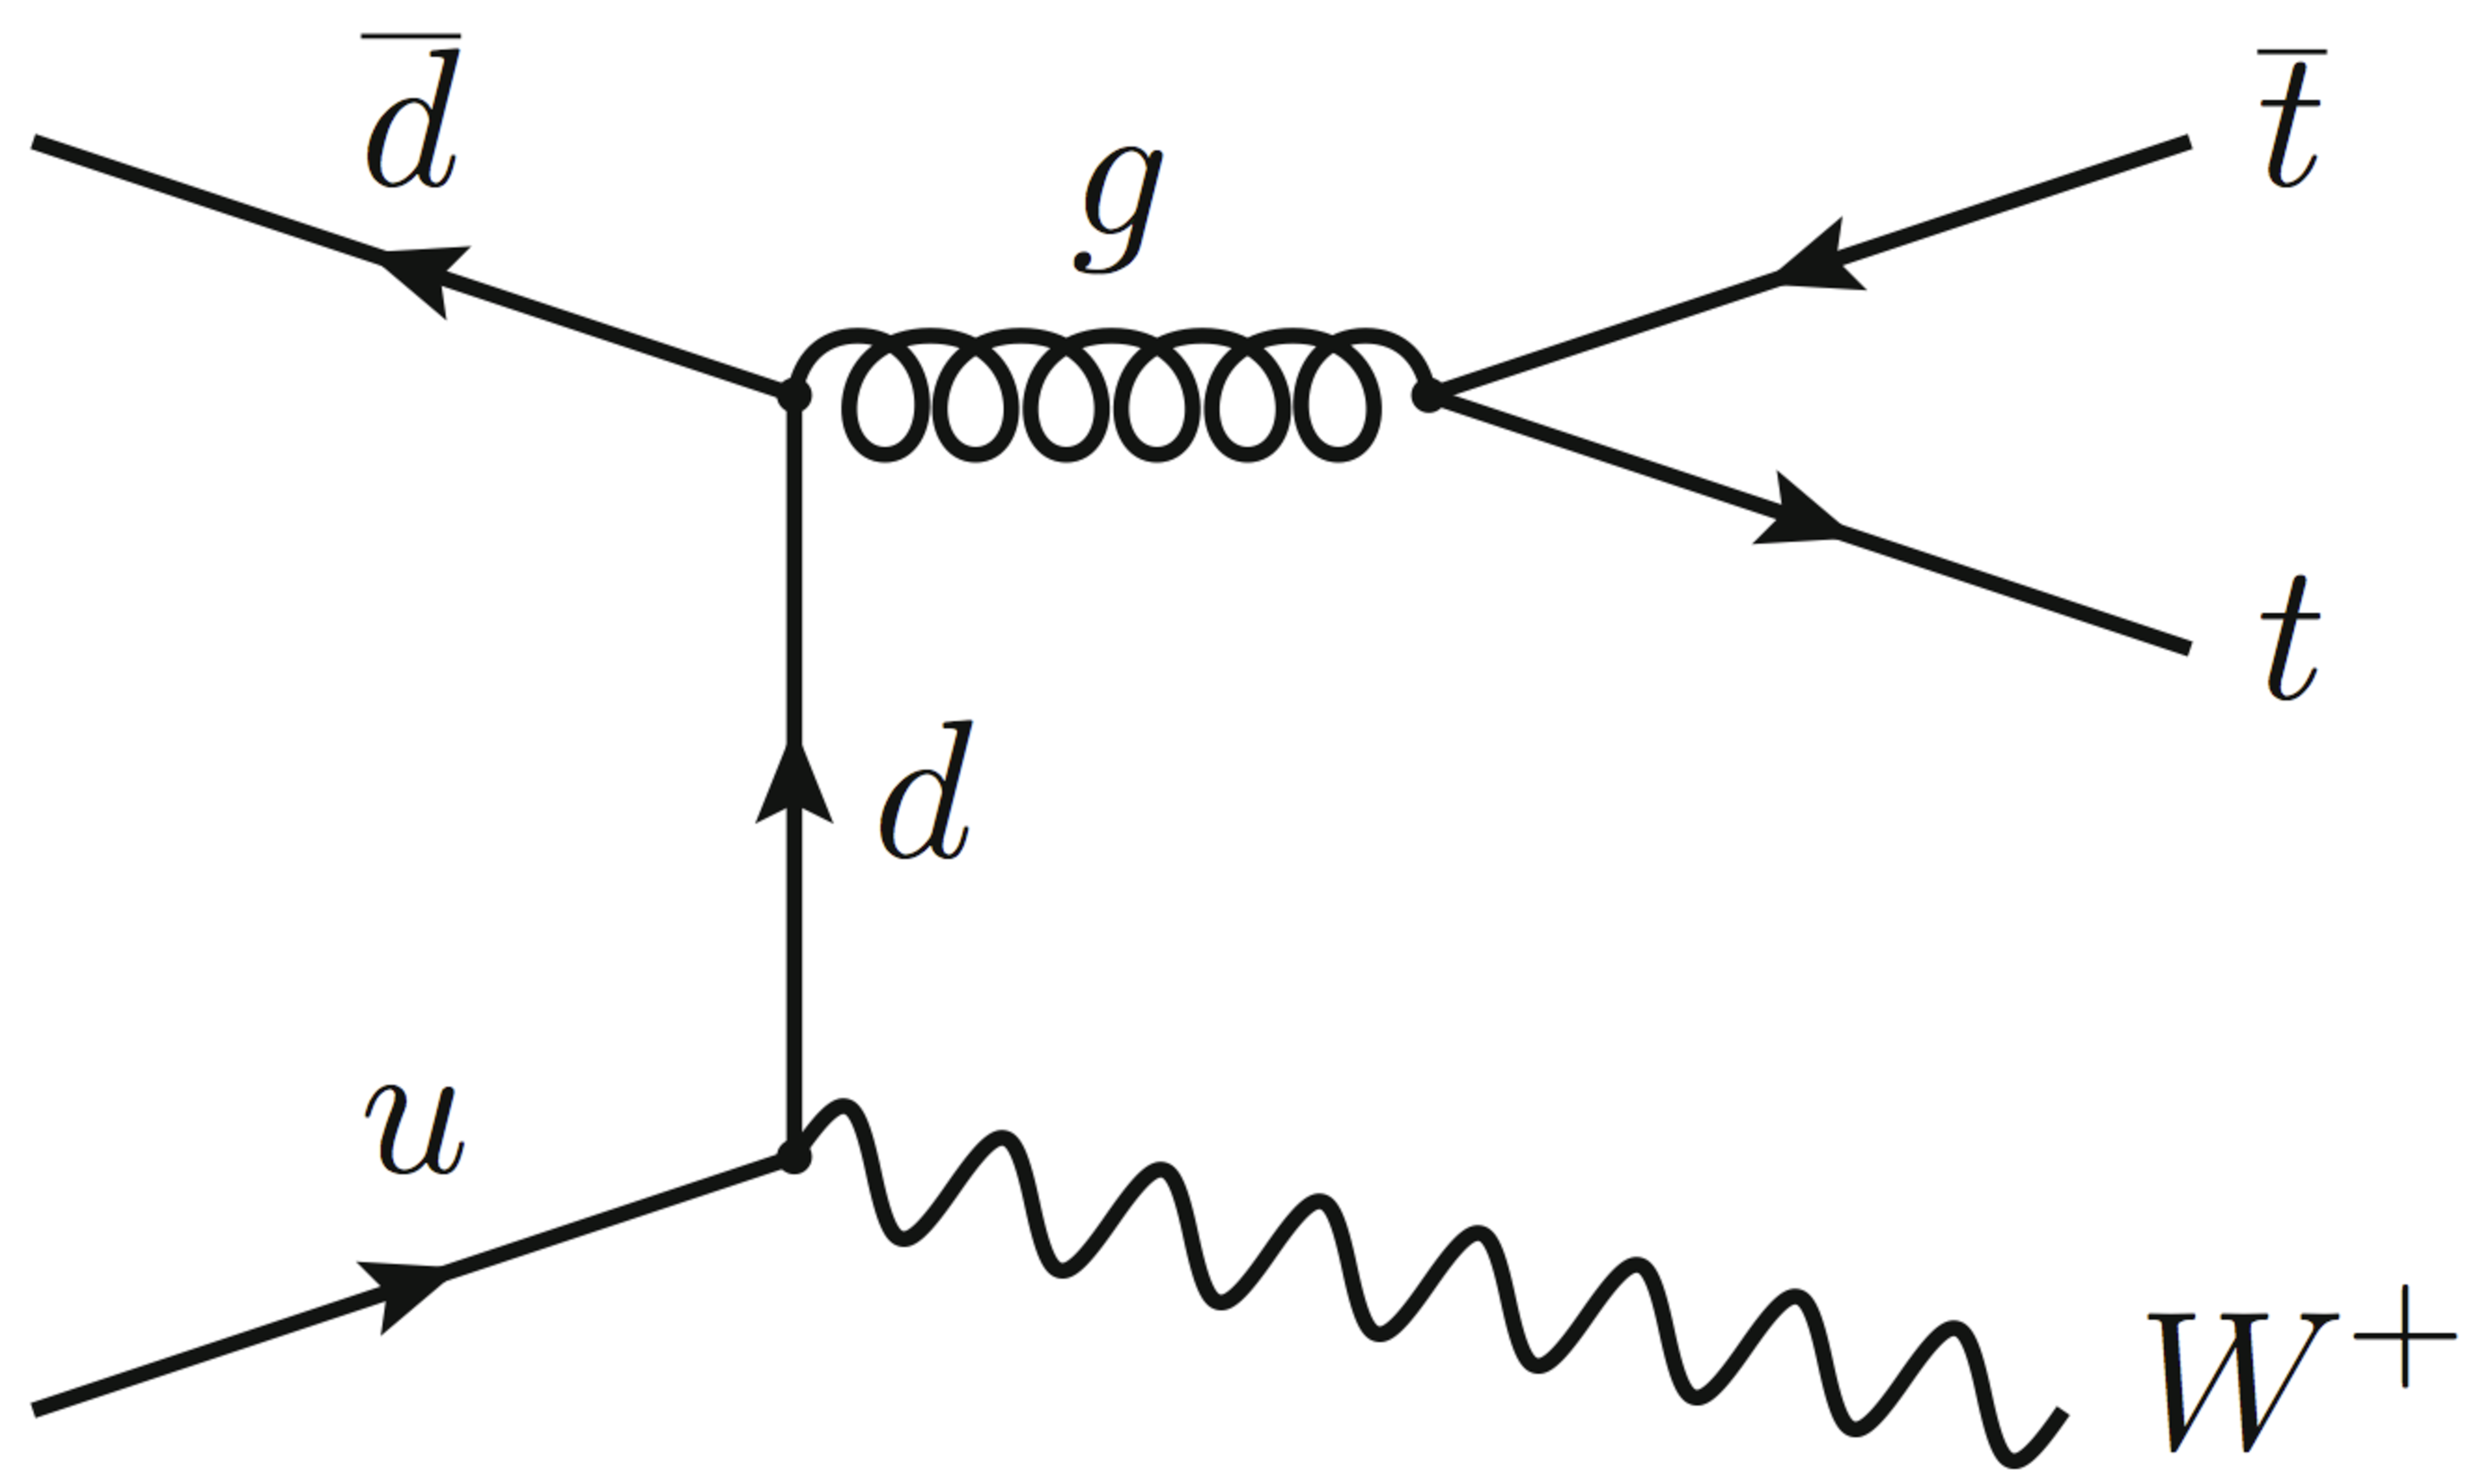
\includegraphics[scale=0.1]{ttW_feynman.pdf}
    \vspace{3mm}
    \caption{}
    \label{fig:ttV}
    % https://twiki.cern.ch/twiki/bin/view/CMSPublic/PhysicsResultsTOP14021
\end{figure}
\clearpage
%%\chapter{Event Selection and Background Estimation} % Main chapter title
\section{Diboson}
\label{SectionDibosons} % For referencing the chapter elsewhere, use \ref{Chapter1} 



%%%%%%%%%%%%%%%%%%%%%%%%%%%%%%%%%%%%%%%%%%%%%%%%%%%%%%%%%%%%
\subsection{LO diagrams for WW production} 
%%%%%%%%%%%%%%%%%%%%%%%%%%%%%%%%%%%%%%%%%%%%%%%%%%%%%%%%%%%%

\vspace{7mm}

\begin{figure}[htb]
    \centering
    \begin{fmffile}{WWschannel}
    \begin{fmfgraph*}(100,80)
    % # in/out
    \fmfleft{i1,i2}
    \fmfright{o1,o2}    
    % ins
    \fmf{fermion}{i1,v1}
    \fmf{fermion}{v1,i2}
    \fmflabel{\(q\)}{i1}
    \fmflabel{\(\overline{q}'\)}{i2}
    % mediators    
    \fmf{photon, label=$Z^0~/~\gamma^*$}{v1,v2}
    % outs
    \fmf{photon}{v2,o1}
    \fmflabel{$W^+$}{o1}
    \fmf{photon}{v2,o2}
    \fmflabel{$W^-$}{o2}
    \end{fmfgraph*}
    \end{fmffile}
    \vspace{3mm}
    \caption{}
    \label{fig:wwschannel}
    \end{figure}
    
    \vspace{7mm}
    \begin{figure}[htb]
    \centering
    \begin{fmffile}{WWtchannel}
    \begin{fmfgraph*}(100,80)
    % # ins/outs
    \fmfleft{i1,i2}
    \fmfright{o1,o2}
    % ins
    \fmf{plain_arrow}{i1,v1}
    \fmf{plain_arrow}{v2,i2}
    \fmflabel{\(q\)}{i1}
    \fmflabel{\(\overline{q'}\)}{i2}
    % mediators
    \fmf{fermion, label=$\overline{q}''$}{v1,v2}
    % outs
    \fmf{photon}{o1,v1}
    \fmflabel{$W^-$}{o1}
    \fmf{photon}{o2,v2}
    \fmflabel{$W^+$}{o2}
    \end{fmfgraph*}
    \end{fmffile}
    \vspace{3mm}
    \caption{}
    \label{fig:wwtchannel}
    \end{figure}
    \vspace{7mm}
    
    \begin{figure}[htb]
    \centering
    \begin{fmffile}{gg-fusion}
    \begin{fmfgraph*}(100,80)
    % # ins/outs
    \fmfleft{i1,i2}
    \fmfright{o1,o2}
    % ins
    \fmf{gluon}{i1,v1}
    \fmf{gluon}{i2,v2}
    \fmflabel{\(g\)}{i1}
    \fmflabel{\(g\)}{i2}
    %\fmf{gluon,label=$g$,label.dist=5mm}{i2,v2}
    % mediators
    \fmf{plain_arrow, label=$\overline{q}$}{v1,v2}
    \fmf{plain_arrow, label=$q$, label.side=left}{v3,v1}
    \fmf{plain_arrow, label=$q$, label.side=left}{v2,v4}
    \fmf{plain_arrow, label=$\overline{q}'$,label.side=left}{v4,v3}
    % outs
    \fmf{photon}{o1,v3}
    \fmflabel{$W^-$}{o1}
    \fmf{photon}{o2,v4}
    \fmflabel{$W^+$}{o2}
    \end{fmfgraph*}
    \end{fmffile}
    \vspace{3mm}
    \caption{}
    \label{fig:ggfusion}
    \end{figure}
    \vspace{7mm}

%%%%%%%%%%%%%%%%%%%%%%%%%%%%%%%%%%%%%%%%%%%%%%%%%%%%%%%%%%%%
\subsection{LO diagrams for WZ production} 
%%%%%%%%%%%%%%%%%%%%%%%%%%%%%%%%%%%%%%%%%%%%%%%%%%%%%%%%%%%%


\vspace{7mm}
% qq-> WZ
% ============
%  s-channel  
% ============
\begin{figure}[htb]
%\subfigure[s-channel]{
\centering
\begin{fmffile}{schannel}
  \begin{fmfgraph*}(100,80)
    % # in/out
    \fmfleft{i1,i2}
    \fmfright{o1,o2}    
    % ins
    \fmf{fermion}{i1,v1}
    \fmf{fermion}{v1,i2}
    \fmflabel{\(q\)}{i1}
    \fmflabel{\(\overline{q}'\)}{i2}
    % mediators    
    \fmf{photon, label= $W^{\pm}$}{v1,v2}
    % outs
    \fmf{photon}{v2,o1}
    \fmflabel{$W^{\pm}$}{o1}
    \fmf{photon}{v2,o2}
    \fmflabel{$Z^0$}{o2}
\end{fmfgraph*}
\end{fmffile}
\vspace{3mm}
%}
\caption{}
\label{fig:WZ_schannel}
\end{figure}
\vspace{7mm}

% ============
%  t-channel  
% ============
\begin{figure}[htb]
%\subfigure[t-channel]{
\centering
\begin{fmffile}{tchannel}
  \begin{fmfgraph*}(100,80)
    % # in/out
     \fmfbottom{i1,d1,o1}
    \fmftop{i2,d2,o2}
    %\fmfleft{i1,i2}
    %\fmfright{o1,o2}
    % ins     
    \fmf{plain_arrow}{i1,v1}
    \fmf{plain_arrow}{v2,i2}
    \fmflabel{\(q\)}{i1}
    \fmflabel{\(\overline{q}'\)}{i2}
    % mediators
    \fmf{fermion, label=$q'$, label.side=left, tension=0}{v1,v2}
    % outs
    \fmf{photon}{o1,v1}
    \fmflabel{$W^{\pm}$}{o1}
    \fmf{photon}{o2,v2}
    \fmflabel{$Z^0$}{o2}
   \end{fmfgraph*}
   %\hspace{2em}
\end{fmffile}
\vspace{3mm}
%}
\caption{}
\label{fig:WZ_tchannel}
\end{figure}
\vspace{7mm}

% ============
%  u-channel  
% ============
\begin{figure}[htb]
%\subfigure[u-channel]{
\centering
\begin{fmffile}{uchannel}
  \begin{fmfgraph*}(100,80)
    %\fmfleft{i1,i2}
    %\fmfright{o1,o2}
  
    % # in/out
    \fmfstraight
    \fmfbottom{i1,v1,o1}
    \fmftop{i2,v2,o2}    
    % ins
    \fmf{fermion, tension= 1/1.5}{i1,v1}
    \fmf{fermion, tension= 1/1.5}{v2,i2}
    \fmflabel{\(q\)}{i1}
    \fmflabel{\(\overline{q}'\)}{i2}
    % mediators    
    \fmf{fermion, label=$q$, label.side=left, tension=0.2}{v1,v2}
    % outs
    \fmf{photon, tension=0.2}{v1,o2}
    \fmflabel{$W^{\pm}$}{o1}
    \fmf{photon, tension=0.2}{v2,o1}
    \fmflabel{$Z^0$}{o2}
\end{fmfgraph*}
\end{fmffile}
\vspace{3mm}
%}
\caption{}
\label{fig:WZ_uchannel}
\end{figure}
\vspace{7mm}

% ===============
%  ZZ-> 2l2nu o ZZ->2l2Q
% ===============

%%%%%%%%%%%%%%%%%%%%%%%%%%%%%%%%%%%%%%%%%%%%%%%%%%%%%%%%%%
\section{LO diagrams for ZZ Production} 
%%%%%%%%%%%%%%%%%%%%%%%%%%%%%%%%%%%%%%%%%%%%%%%%%%%%%%%%%%


\vspace{7mm}

% ===============
%  qq'-> ZZ
% ===============
\begin{figure}[htb]
\centering
\begin{fmffile}{qqZZ}
\begin{fmfgraph*}(100,80)
    % # ins/outs
    \fmfleft{i1,i2}
    \fmfright{o1,o2}
    % ins
    \fmf{plain_arrow}{i1,v1}
    \fmf{plain_arrow}{v2,i2}
    \fmflabel{\(q\)}{i1}
    \fmflabel{\(\overline{q}\)}{i2}
    % mediators
    \fmf{fermion, label=$q$}{v1,v2}
    % outs
    \fmf{photon}{o1,v1}
    \fmflabel{$Z$}{o1}
    \fmf{photon}{o2,v2}
    \fmflabel{$Z$}{o2}
\end{fmfgraph*}
\end{fmffile}
\vspace{3mm}
%}
\caption{}
\label{fig:qqZZ}
\end{figure}
\vspace{7mm}

% ===============
%  gg-> ZZ
% ===============
\begin{figure}[htb]
%\subfigure[(b)]{
\centering
   \begin{fmffile}{ggZZ}
   \begin{fmfgraph*}(100,80)
    % # ins/outs
    \fmfleft{i1,i2}
    \fmfright{o1,o2}
    % ins
    \fmf{gluon}{i1,v1}
    \fmf{gluon}{i2,v2}
    \fmflabel{\(g\)}{i1}
    \fmflabel{\(g\)}{i2}
    %\fmf{gluon,label=$g$,label.dist=5mm}{i2,v2}
    % mediators
    \fmf{plain_arrow, label=$q$}{v1,v2}
    \fmf{plain_arrow, label=$\overline{q}$, label.side=left}{v3,v1}
    \fmf{plain_arrow, label=$q$, label.side=left}{v2,v4}
    \fmf{plain_arrow, label=$\overline{q}$,label.side=left}{v4,v3}
    % outs
    \fmf{photon}{o1,v3}
    \fmflabel{$Z$}{o1}
    \fmf{photon}{o2,v4}
    \fmflabel{$Z$}{o2}
    \end{fmfgraph*}
    \end{fmffile}
%}
\vspace{3mm}
\caption{}
\label{fig:ggZZ}
\end{figure}
\vspace{7mm}


\clearpage
%\section{Drell-Yan Background} % Main chapter title

\label{SectionDY} % For referencing the chapter elsewhere, use \ref{Chapter1} 


%%%%%%%%%%%%%%%%%%%%%%%%%%%%%%%%%%%%%%%%%%%%%%%%%%%%%%%%%%%%
\subsection{LO diagrams for Drell-Yan plus jets (Z+jets) production} 
%%%%%%%%%%%%%%%%%%%%%%%%%%%%%%%%%%%%%%%%%%%%%%%%%%%%%%%%%%%%

\vspace{7mm}

\begin{figure}[htb]
\centering
    \begin{fmffile}{DYLO}
      \begin{fmfgraph*}(100,80)
      % # ins/outs
      \fmfleft{i1,i2}
      \fmfright{o1,o2}
      % ins
      \fmf{fermion}{i2,v1}
      \fmf{fermion}{v1,i1}
      % mediators
      \fmf{photon, label=$Z^0/\gamma^*$}{v1,v2}
      % outs
      \fmf{fermion}{v2,o2}
      \fmf{fermion}{o1,v2}
      % labels
      \fmflabel{$q$}{i2}
      \fmflabel{$\overline{q}$}{i1}
      \fmflabel{$\ell^-$}{o2}
      \fmflabel{$\ell^+$}{o1}
      %\fmflabel{$\ell^- /~ q'$}{o2}
      %\fmflabel{$\ell^+ /~ \overline{q}'$}{o1}
      \end{fmfgraph*}
    \end{fmffile}
    \vspace{3mm}
    \caption{}
    \label{fig:DYLO}
    \end{figure}
    \vspace{7mm}
    
     \begin{figure}[htb]
    \centering
    \begin{fmffile}{DYLO-tchannel}
      \begin{fmfgraph*}(100,80)
       % # ins/outs
      \fmfstraight
      \fmftop{i2,v2,o2}
      \fmfbottom{i1,v1,o1}
      % ins
      \fmf{fermion}{i2,v2}
      \fmf{fermion}{v1,i1}
      % mediators
      \fmf{photon, label=$Z^0/\gamma^*$}{v1,v2}
      % outs
      \fmf{fermion}{v2,o2}
      \fmf{fermion}{o1,v1}
      % labels
      \fmflabel{$q'$}{i2}
      \fmflabel{$\overline{q}$}{i1}
      \fmflabel{$q'$}{o2}
      \fmflabel{$\overline{q}$}{o1} 
      \fmfdotn{v}{2}
      \end{fmfgraph*}
    \end{fmffile}
    \vspace{3mm}
    \caption{}
    \label{fig:DYLO_tchannel}
    \end{figure}
    \vspace{7mm}
    
    \begin{figure}[htb]
    \centering
    \begin{fmffile}{DYjets}
      \begin{fmfgraph*}(100,80)
      \fmfleft{i2,i1}
      \fmfright{o2,o1}
      \fmftop{t}
      \fmf{phantom}{i1,v1,i2}
      \fmf{phantom}{o1,v2,o2}
      \fmf{phantom}{v1,v2}
      \fmffreeze
      \fmf{fermion}{i1,g}
      \fmf{plain,tension=2.8}{g,v1}
      \fmf{fermion}{v1,i2}
      \fmf{gluon,tension=0}{t,g}
      \fmf{boson,label=$Z^0 /\gamma^*$,label.side=right}{v1,v2}
      \fmf{fermion}{o2,v2,o1}
      \fmflabel{$q$}{i1}
      \fmflabel{$\overline{q}$}{i2}
      \fmflabel{$\ell^+$}{o2}
      \fmflabel{$\ell^-$}{o1}
      %\fmflabel{$\ell^- /~ q'$}{o2}
      %\fmflabel{$\ell^+ /~ \overline{q}'$}{o1}
      \end{fmfgraph*}
    \end{fmffile}
    \vspace{3mm}
    \caption{}
    \label{fig:DYjets_LO}
    %https://wiki.physik.uzh.ch/cms/latex:feynman
    \end{figure}
    \vspace{7mm}
    
    \begin{figure}[htb]
    \centering
    \begin{fmffile}{Z+jets}
      \begin{fmfgraph*}(100,80)
      \fmfleft{i2,i1} 
      \fmfright{o2,o1}
      \fmf{fermion}{i1,v1}
      \fmf{fermion}{v2,i2}
      \fmf{fermion, label=$q$}{v1,v2}
      \fmf{photon}{v1,o1}
      \fmf{gluon}{v2,o2}
      \fmflabel{$q$}{i1}
      \fmflabel{$\overline{q}$}{i2}
      \fmflabel{$g$}{o2}
      \fmflabel{$Z^0$}{o1}
      \end{fmfgraph*}
    \end{fmffile}
    \vspace{3mm}
    \caption{}
    \label{fig:Z+jets_LO}
    %https://wiki.physik.uzh.ch/cms/latex:feynman
    \end{figure}
\vspace{7mm}


\begin{figure}[htb]
    \centering
    \begin{fmffile}{Zdecays}
    \begin{fmfgraph*}(100,80)
    % # ins/out
    \fmfleft{i1}
    \fmfright{o1,o2}
    % mediators
    \fmf{photon, label=$Z$}{i1,v1}
    % outs
    \fmf{fermion}{v1,o1}
    \fmflabel{$\ell^- / q /\nu $}{o1}
    \fmf{fermion}{o2,v1}
    \fmflabel{$\ell^+ / \overline{q} /\overline{\nu} $}{o2}
    \end{fmfgraph*}
    \end{fmffile}
    \vspace{4mm}
    \caption{}
    \label{fig:Zdecays}
\end{figure}
\clearpage
%\section{Higgs Backgrounds}
\label{SectionHiggs}
%%%%%%%%%%%%%%%%%%%%%%%%%%%%%%%%%%%%%%%%%%%%%%%%%%%%%%%%%%
In a proton-proton collision the Higgs boson can be produced in different ways:
via gluon-gluon fusion, the vector boson fusion (VBF), the vector-boson associated
production (Higgs Strahlung) and the top-quark associated production.

\subsection{LO diagrams for Higgs Production} 
%%%%%%%%%%%%%%%%%%%%%%%%%%%%%%%%%%%%%%%%%%%%%%%%%%%%%%%%%%
LO production of Higgs process at the LHC collider in Figure~\ref{fig:Higgs}
\vspace{5mm}

\begin{figure}[h]
%\scalebox{0.9}[0.9]{ 
 \centering
% ===============
% Higgs strahlung: q q' -> W*,Z*-> H W,Z
% ===============
\begin{subfigure}[ht]{0.45\textwidth}
%\subfigure[(a)]{
\centering
\begin{fmffile}{qqHWZ}
\begin{fmfgraph*}(100,80)
  % # in/out
  \fmfleft{i1,i2}
  \fmfright{o1,o2}
  % ins
  \fmf{fermion}{v1,i1}
  \fmf{fermion}{i2,v1}
  \fmflabel{\(\overline{q}\)}{i1}
  \fmflabel{\(q'\)}{i2}
  % mediators
  \fmf{photon, label= $W^{*};Z^{*}$}{v1,v2}
  % outs
  \fmf{photon}{v2,o1}
  \fmf{dashes}{v2,o2}
  \fmflabel{\(W;Z\)}{o1}
  \fmflabel{\(H\)}{o2}
  \end{fmfgraph*} 
  \end{fmffile}
%}
\vspace{3mm}
\caption{Higgs Strahlung}
\label{fig:qqHWZ}
\end{subfigure}
\vspace{3mm}
%\hspace{3mm}
% =========================
% Vector boson fusion: W,Z
% =========================
\begin{subfigure}[ht]{0.45\textwidth}
%\subfigure[(b)]{
\centering
\begin{fmffile}{VBFHWZ}
\begin{fmfgraph*}(100,80)
  % # in/out
  \fmfleft{i1,i2}
  \fmfright{o1,o2,o3}
  % ins
  \fmf{fermion}{i1,v1}
  \fmf{fermion}{i2,v2}
  \fmflabel{\(q\)}{i1}
  \fmflabel{\(q'\)}{i2}
  % mediators
  \fmf{photon, label= $W ;Z$}{v1,v3}
  \fmf{photon, label= $W ;Z$ , label.side=left}{v2,v3}
  % outs
  \fmf{fermion}{v1,o1}
  \fmf{dashes}{v3,o2}
  \fmf{fermion}{v2,o3}
  %\fmflabel{\(W;Z\)}{o1}
  \fmflabel{\(H\)}{o2}
\end{fmfgraph*}
\end{fmffile}
%}
\vspace{3mm}
\caption{VBF}
\label{fig:qqVBFH}
\end{subfigure}
\vspace{3mm}
%\hspace{3mm}

% =========================
%  ttH (\ttbar H)
% =========================
\begin{subfigure}[hb]{0.45\textwidth}
%\subfigure[(c)]{
\centering
\begin{fmffile}{ttH}
\begin{fmfgraph*}(100,80)
  % # in/out
  \fmfleft{i1,i2}
  \fmfright{o1,o2,o3}
  % ins
  \fmf{gluon}{i1,v1}
  \fmf{gluon}{i2,v2}
  \fmflabel{\(g\)}{i1}
  \fmflabel{\(g\)}{i2}
  % mediators
  \fmf{plain_arrow, label= $t$}{v1,v3}
  \fmf{plain_arrow, label= $\overline{t}$}{v3,v2}
  % outs
  \fmf{fermion, label=$\overline{t}$}{o1,v1}
  %\fmflabel{$\overline{t}$}{o1}
  \fmf{fermion, label=$t$, label.side=left}{v2,o3}
  %\fmflabel{$t$}{o3}
  \fmf{dashes}{v3,o2}
  \fmflabel{\(H\)}{o2}
\end{fmfgraph*}
\end{fmffile}
%}
\vspace{3mm}
\caption{Top-quark associated production}
\label{fig:ttH}
\end{subfigure}
\vspace{3mm}
%\hspace{3mm}
% =========================
%  ttH (\ttbar H) v2
% =========================
\begin{subfigure}[hb]{0.45\textwidth}
%\subfigure[(d)]{
\centering
\begin{fmffile}{ggFusion}
\begin{fmfgraph*}(100,80)
  % # in/out
  \fmfleft{i1,i2}
  \fmfright{o1}
  % ins
  \fmf{gluon}{i1,v1}
  \fmf{gluon}{i2,v2}
  \fmflabel{\(g\)}{i1}
  \fmflabel{\(g\)}{i2}
  % mediators
  %\fmfpoly{triangle, empty}{v1,v2,v3}
  %\fmf{phantom}{v1,v2,v3}
  \fmf{fermion, tension=1/1.5, label= $t$}{v1,v2}
  \fmf{fermion, tension=1/1.5, label= $t$, label.side=left}{v2,v3}
  \fmf{fermion, tension=1/1.5, label= $\overline{t}$}{v3,v1}
  % outs
  \fmf{dashes}{v3,o1}
  \fmflabel{\(H\)}{o1}
\end{fmfgraph*}
\end{fmffile}
%}
\vspace{3mm}
\caption{Gluon-gluon fusion}
\label{fig:ggFusion}
\end{subfigure}
%}
\vspace{3mm}
%\hspace{3mm}
\caption{Higgs Production LO }
% https://arxiv.org/pdf/1610.07922.pdf
\label{fig:Higgs}
\end{figure}
\clearpage
%\section{Triboson Background}
\label{SectionTriboson}

\vspace{7mm}

\begin{figure}[htb]
    \centering
    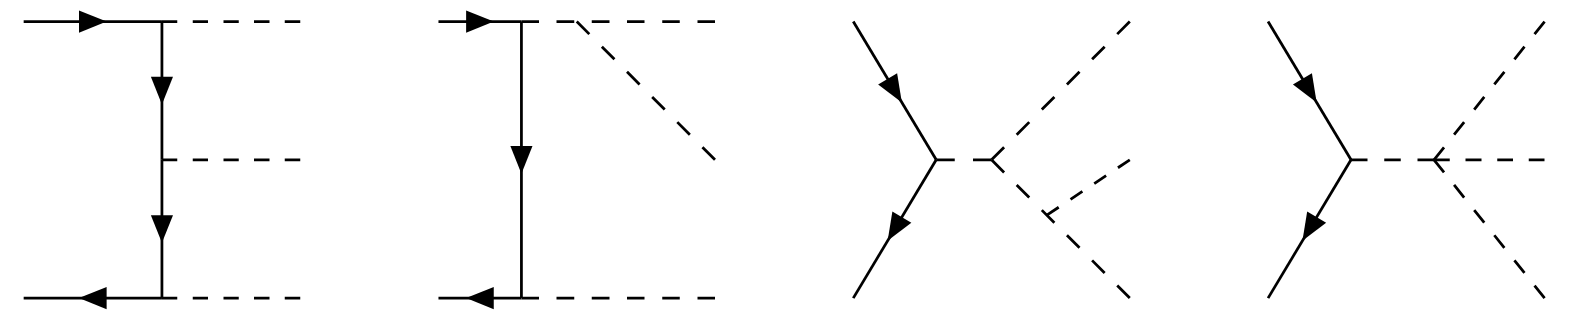
\includegraphics[scale=0.2]{TribosonGeneric.png}
    \caption{}
    % https://www.ugr.es/~pittau/talk_granada_2008.pdf
    \label{fig:TriGeneric}
\end{figure}


A representative example of each process is shown in next sections. 

The qq-> VVV production is dominant with respect the gluon production


\subsection{An example of WWW production}

\vspace{7mm}

\begin{figure}[htb]
    \centering
    \begin{fmffile}{WWW}
    \begin{fmfgraph*}(100,60)
      % # ins/outs
      \fmfleft{i1,i2}
      \fmfright{o1,o2,o3}
      \fmftop{t}
      \fmfbottom{b}
      % ins
      \fmf{fermion}{i2,v1}
      \fmf{fermion}{v1,i1}
      % mediators
      \fmf{photon, label=$W^{\pm}$}{v1,v2}
      \fmf{photon}{v2,o2}
      \fmflabel{$W^{\mp}$}{o2}
      \fmffreeze
      \fmf{phantom}{v2,o1}
      %\fmf{phantom}{v2,o2}
      \fmf{phantom}{v2,o3}
      \fmffreeze
      \fmf{photon,tension=0}{v2,o1}
      \fmf{photon,tension=0}{v2,o3}
      % labels
      \fmflabel{$q$}{i2}
      \fmflabel{$\overline{q}'$}{i1}
      \fmflabel{$W^{\pm}$}{o3}
      \fmflabel{$W^{\pm}$}{o1}
    \end{fmfgraph*}
    \end{fmffile}
    \vspace{3mm}
    \caption{}
    \label{fig:WWW}
    % https://open.bu.edu/handle/2144/17737
\end{figure}



\subsection{An example of WWZ production}


\vspace{7mm}


\begin{figure}[htb]
    \centering
    \begin{fmffile}{WWZ}
    \begin{fmfgraph*}(100,60)
    \fmfstraight
    \fmfleft{i2,i1}
    \fmfright{o1,l1,l2}
    % skeleton
    \fmf{phantom}{i1,v1}
    \fmf{phantom}{v1,l1}
    \fmf{phantom, tension=0.3}{v1,v2}
    \fmf{phantom}{i2,v2}
    \fmf{phantom}{v2,o1}
    \fmffreeze
    % W + jets
    \fmfshift{5 right}{l1,l2}
    \fmfshift{20 left}{o1}
    % quarks
    \fmflabel{$q$}{i1}
    \fmflabel{$\overline{q}$}{i2}
    \fmf{fermion}{i1,v1,v2,i2}
    % W boson
    \fmf{boson,tension=1.2,label=$Z^0/\gamma$,label.side=left}{v1,z}
    \fmf{photon}{v2,o1}
    \fmflabel{$Z^0$}{o1}
    % leptons
    \fmflabel{$W^+$}{l1}
    \fmflabel{$W^-$}{l2}
    \fmf{photon}{l1,z,l2}
    \end{fmfgraph*}
    \end{fmffile}
    \vspace{3mm}
    \caption{}
    \label{fig:WWZ}
\end{figure}

% https://arxiv.org/pdf/1310.6159.pdf

\subsection{An example of WZZ production}
\vspace{7mm}

\begin{figure}[htb]
    \centering
    \begin{fmffile}{WZZ}
    \begin{fmfgraph*}(100,60)
    %\fmfstraight
    \fmfleft{i1,i3} 
    \fmfright{o1,o2,o3}
    \fmf{fermion}{v1,i1}
    \fmf{fermion}{i3,v3}
    \fmf{photon}{v3,o3}
    \fmf{photon}{v1,o1}
    \fmffreeze
    \fmf{fermion, label.side=left}{v3,v2,v1}
    \fmffreeze
    \fmf{photon, tension= 1.1}{v2,o2}
    \fmflabel{$\overline{q}$}{i1}
    \fmflabel{$q$'}{i3}
    \fmflabel{$W^{\pm}$}{o2}
    \fmflabel{$Z^0$}{o1}
    \fmflabel{$Z^0$}{o3}
    \end{fmfgraph*}
    \end{fmffile}
    \vspace{3mm}
    \caption{}
    \label{fig:WZZ}
\end{figure}

\subsection{An example of ZZZ production}

\vspace{7mm}

\begin{figure}[htb]
    \centering
    \begin{fmffile}{ZZZ}
  \begin{fmfgraph*}(100,60)
    \fmfstraight
    \fmfleft{i2,m,i1}
    \fmfright{o2,l2,l1}
    % skeleton
    \fmf{phantom,tension=1.0}{i1,v1}
    \fmf{phantom,tension=1.0}{v2,l1}
    \fmf{phantom,tension=1.5}{v1,v2}
    \fmf{phantom,tension=1.0}{i2,v1}
    \fmf{phantom,tension=1.0}{v2,o2}
    \fmf{phantom,tension=0.6}{i1,t1,m}
    \fmf{phantom,tension=0.6}{t1,LQ}
    \fmf{phantom,tension=2.0}{l1,LQ,l2}
    \fmffreeze
    % gluon + quarks
    \fmf{phantom,tension=5.0}{i1,g} % shorten leg
    \fmf{phantom,tension=5.0}{i2,q} % shorten leg
    \fmf{phantom,tension=5.0}{o2,l} % shorten leg
    \fmf{fermion}{g,v1}
    \fmf{fermion}{v1,q}
    \fmf{photon,label=$Z^0$,label.side=right}{v1,v2}
    \fmf{photon}{v2,l}
    \fmflabel{$q$}{g}
    \fmflabel{$\overline{q}$}{q}
    \fmflabel{$Z^0$}{l}
    % LQ
    \fmf{dashes,tension=1.2,label=H,label.side=left}{v2,LQ}
    % LQ -> lepton + quark
    \fmf{photon}{l2,LQ,l1}
    \fmfshift{20 right}{l1,l2}
    \fmflabel{$Z^0$}{l1}
    \fmflabel{$Z^0$}{l2}
  \end{fmfgraph*}
\end{fmffile}
\vspace{3mm}
    \caption{}
    \label{fig:ZZZ}
\end{figure}
\clearpage
%\section{Fakes}
\label{SectionFakes}

\subsection{W+jets Production}


\vspace{7mm}


    \begin{figure}[htb]
    \centering
    \begin{fmffile}{Wjetsa}
  \begin{fmfgraph*}(100,100)
    \fmfstraight
    \fmfleft{i2,i1}
    \fmfright{o1,l2,l1}
    % skeleton
    \fmf{phantom,tension=1.8}{i1,v1}
    \fmf{phantom,tension=1.0}{v1,l1}
    \fmf{phantom,tension=1.8}{v1,v2}
    \fmf{phantom,tension=1.8}{i2,v2}
    \fmf{phantom,tension=1.0}{v2,o1}
    \fmffreeze
    % W + jets
    \fmfshift{5 right}{l1,l2}
    \fmfshift{20 left}{o1}
    % quarks
    \fmflabel{$q$}{i1}
    \fmflabel{$\overline{q}$}{i2}
    \fmf{fermion}{i1,v1,v2,i2}
    % W boson
    \fmf{boson,tension=1.2,label=$W^\pm$,label.side=left}{v1,z}
    \fmf{gluon}{v2,o1}
    % leptons
    \fmflabel{$\ell^\pm$}{l1}
    \fmflabel{$\nu_\ell/~\overline{\nu}_\ell$}{l2}
    \fmf{fermion}{l1,z,l2}
  \end{fmfgraph*}
\end{fmffile}
    \vspace{3mm}
    \caption{}
    \label{fig:Wjetsa}
    \end{figure}
    \vspace{7mm}
    
    \begin{figure}[htb]
    \centering
    \begin{fmffile}{Wjetsb}
    \begin{fmfgraph*}(100,100)
    \fmfleft{i2,i1}
    \fmfright{o2,o1}
    \fmftop{t}
    \fmf{phantom}{i1,v1,i2}
    \fmf{phantom}{o1,v2,o2}
    \fmf{phantom}{v1,v2}
    \fmffreeze
    \fmf{fermion}{i1,g}
    \fmf{plain,tension=2.8}{g,v1}
    \fmf{fermion}{v1,i2}
    \fmf{gluon,tension=0}{t,g}
    \fmf{boson,label=$W^{\pm}$,label.side=right}{v1,v2}
    \fmf{fermion}{o2,v2,o1}
    \fmflabel{$q$}{i1}
    \fmflabel{$\overline{q}$}{i2}
    \fmflabel{$\ell^\pm$}{o1}
    \fmflabel{$\nu_\ell/~\overline{\nu}_\ell$}{o2}
    \end{fmfgraph*}
    \end{fmffile}
    \vspace{3mm}
    \caption{}
    \label{fig:Wjetsb}
    \end{figure}
    \vspace{7mm}
    

%%%%%%%%%%%%%%%%%%%%%%%%%%%%%%%%%%%%%%%%%%%%%%%%%%%%%%%%%%%%
\subsection{ ttbar semileptonic} 
%%%%%%%%%%%%%%%%%%%%%%%%%%%%%%%%%%%%%%%%%%%%%%%%%%%%%%%%%%%%


\vspace{7mm}

 \begin{figure}[htb]
 \centering
 \begin{fmffile}{tt1l}
  \begin{fmfgraph*}(180,150)
    \fmfset{arrow_len}{3.5mm}
    \fmfstraight
    \fmfleft{i1,i2,i3,i4,i5}
    \fmfright{o1,o2,o3,o4,o5,o6}
    % bW -> bqq
    \fmf{boson,tension=1.5,label={$W^+$},label.side=right}{v2,v21}  % W boson
    \fmf{fermion}{v2,o6}     % b quark
    \fmf{fermion}{o5,v21,o4}
    % bW -> blnu
    \fmf{boson,tension=1.5,label={$W^-$},label.side=right}{v1,v11}  % W boson
    \fmf{fermion}{o3,v1}     % b quark
    \fmf{fermion}{o1,v11,o2}
    \fmf{fermion,tension=1.5}{v1,i3,v2}  % top quark pair
    \fmf{phantom,label={$\overline{t}$},tension=1,label.side=rigth}{i3,v1}
    \fmf{phantom,label={$t$},tension=1,label.side=left}{i3,v2}
    \fmflabel{$\overline{\nu}_{\ell}  $}{o1}
    \fmflabel{$ \ell^-$}{o2}
    \fmflabel{$\overline{b}$}{o3}
    \fmflabel{$q$}{o4}
    \fmflabel{$\overline{q}'$}{o5}
    \fmflabel{$b$}{o6}
  \end{fmfgraph*}
\end{fmffile}

\vspace{3mm}
    \caption{}
    \label{fig:ttbarsemiLep}
\end{figure}
\clearpage
%%\chapter{Event Selection and Background Estimation} % Main chapter title
\section{Higgs couplings}
\label{HiggsCouplings} % For referencing the chapter elsewhere, use \ref{Chapter1} 



%%%%%%%%%%%%%%%%%%%%%%%%%%%%%%%%%%%%%%%%%%%%%%%%%%%%%%%%%%%%
\subsection{Three lowest-order Feynman diagrams for Higgs decay} 
%%%%%%%%%%%%%%%%%%%%%%%%%%%%%%%%%%%%%%%%%%%%%%%%%%%%%%%%%%%%


\vspace{7mm}

\begin{figure}[h]
    \centering
    \begin{subfigure}[h]{0.45\textwidth}
    \centering
    % coupling to fermions
    \begin{fmffile}{fermions}
    \begin{fmfgraph*}(90,70)
    \fmfleft{i1}
    \fmfright{o1,o2}    
    \fmf{dashes}{i1,v1}
    \fmf{fermion}{o1,v1}
    \fmf{fermion}{v1,o2}
    \fmflabel{$H$}{i1}
    \fmflabel{$\overline{f}$}{o1}
    \fmflabel{$f$}{o2}
    \fmfdotn{v}{1}
    \fmflabel{$m_f\frac{g_W}{2m_W}$}{v1}
    \end{fmfgraph*}
    \end{fmffile}
    \caption{}
    \end{subfigure}
    \begin{subfigure}[h]{0.45\textwidth}
    \centering
     % coupling to W bosons
    \begin{fmffile}{Wboson}
    \begin{fmfgraph*}(90,70)
    \fmfleft{i1}
    \fmfright{o1,o2}    
    \fmf{dashes}{i1,v1}
    \fmf{boson}{o1,v1}
    \fmf{boson}{v1,o2}
    \fmflabel{$H$}{i1}
    \fmflabel{$W^+$}{o1}
    \fmflabel{$W^-$}{o2}
    \fmfdotn{v}{1}
    \fmflabel{$g_W m_W$}{v1}
    \end{fmfgraph*}
    \end{fmffile}
    \caption{}
    \end{subfigure}
    \begin{subfigure}[h]{0.45\textwidth}
    \centering
     % coupling to Z bosons
    \begin{fmffile}{Zboson}
    \begin{fmfgraph*}(90,70)
    \fmfleft{i1}
    \fmfright{o1,o2}    
    \fmf{dashes}{i1,v1}
    \fmf{boson}{o1,v1}
    \fmf{boson}{v1,o2}
    \fmflabel{$H$}{i1}
    \fmflabel{$Z^0$}{o1}
    \fmflabel{$Z^0$}{o2}
    \fmfdotn{v}{1}
    \fmflabel{$m_Z\frac{g_W}{cos\theta_W}$}{v1}
    \end{fmfgraph*}
    \end{fmffile}
    \caption{}
    \end{subfigure}
\label{fig:my_label}
\caption{Lowest order Feynman diagram for three Higgs boson decays.}
\end{figure}


\vspace{7mm}

\begin{fmffile}{feyngraph}
    \begin{fmfgraph*}(100,80)
       \fmfleft{i}
       \fmfright{o}
       \fmfv{label=H,l.a=60}{i}
       \fmfv{label=H,l.a=120}{o}
       \fmf{dashes,tension=1}{i,v1} % ,label=H,label.side=left
       \fmf{dashes,tension=1}{v2,o}
       \fmf{fermion,left,tension=0.4,label=$f$}{v1,v2,v1}
    \end{fmfgraph*}
    \quad  \quad
    \begin{fmfgraph*}(100,80)
       \fmfleft{i}
       \fmfright{o}
       \fmftop{m}
       \fmfv{label=H,l.a=60}{i}
       \fmfv{label=H,l.a=120}{o}
       \fmflabel{$S$}{m}
       \fmf{dashes,tension=1}{i,v1}
       \fmf{dashes,tension=1}{v1,o}
       \fmf{dashes,right,tension=0}{v1,m,v1}
    \end{fmfgraph*}
\end{fmffile}



\end{document}
